% Created by tikzDevice version 0.10.1 on 2017-12-04 16:18:31
% !TEX encoding = UTF-8 Unicode
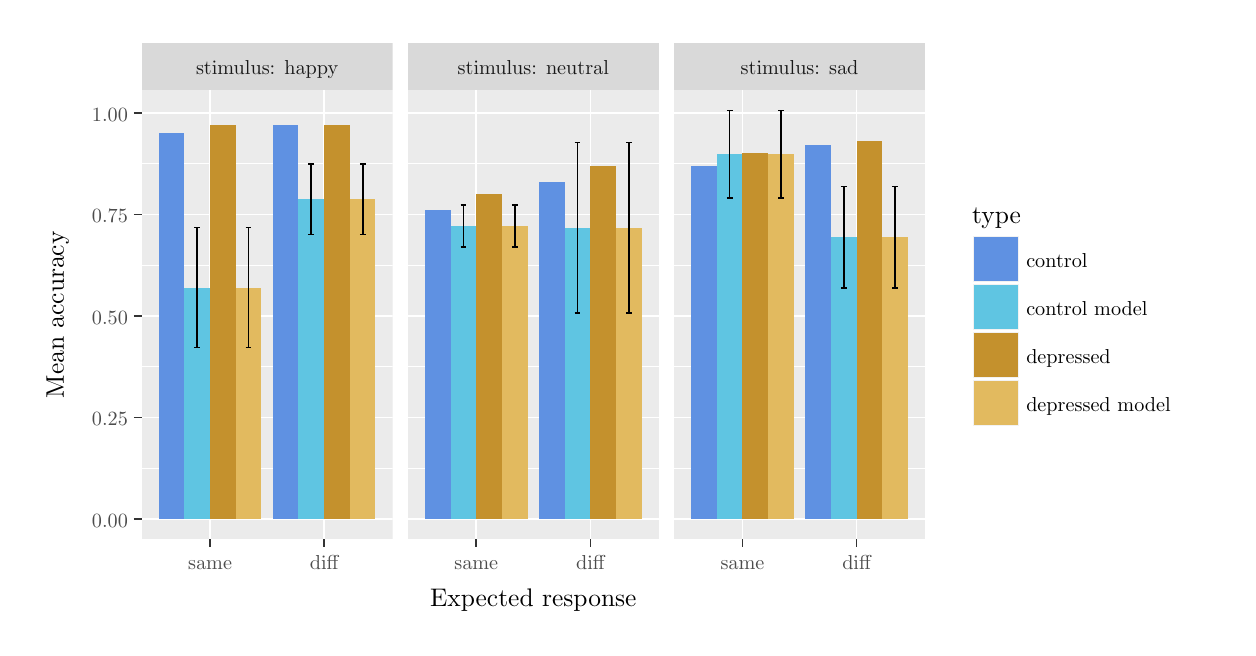
\begin{tikzpicture}[x=1pt,y=1pt]
\definecolor{fillColor}{RGB}{255,255,255}
\path[use as bounding box,fill=fillColor,fill opacity=0.00] (0,0) rectangle (433.62,216.81);
\begin{scope}
\path[clip] (  0.00,  0.00) rectangle (433.62,216.81);
\definecolor{drawColor}{RGB}{255,255,255}
\definecolor{fillColor}{RGB}{255,255,255}

\path[draw=drawColor,line width= 0.6pt,line join=round,line cap=round,fill=fillColor] (  0.00,  0.00) rectangle (433.62,216.81);
\end{scope}
\begin{scope}
\path[clip] ( 41.17, 31.92) rectangle (131.87,194.25);
\definecolor{fillColor}{gray}{0.92}

\path[fill=fillColor] ( 41.17, 31.92) rectangle (131.87,194.25);
\definecolor{drawColor}{RGB}{255,255,255}

\path[draw=drawColor,line width= 0.3pt,line join=round] ( 41.17, 57.64) --
	(131.87, 57.64);

\path[draw=drawColor,line width= 0.3pt,line join=round] ( 41.17, 94.32) --
	(131.87, 94.32);

\path[draw=drawColor,line width= 0.3pt,line join=round] ( 41.17,131.00) --
	(131.87,131.00);

\path[draw=drawColor,line width= 0.3pt,line join=round] ( 41.17,167.68) --
	(131.87,167.68);

\path[draw=drawColor,line width= 0.6pt,line join=round] ( 41.17, 39.30) --
	(131.87, 39.30);

\path[draw=drawColor,line width= 0.6pt,line join=round] ( 41.17, 75.98) --
	(131.87, 75.98);

\path[draw=drawColor,line width= 0.6pt,line join=round] ( 41.17,112.66) --
	(131.87,112.66);

\path[draw=drawColor,line width= 0.6pt,line join=round] ( 41.17,149.34) --
	(131.87,149.34);

\path[draw=drawColor,line width= 0.6pt,line join=round] ( 41.17,186.02) --
	(131.87,186.02);

\path[draw=drawColor,line width= 0.6pt,line join=round] ( 65.91, 31.92) --
	( 65.91,194.25);

\path[draw=drawColor,line width= 0.6pt,line join=round] (107.13, 31.92) --
	(107.13,194.25);
\definecolor{fillColor}{RGB}{226,186,95}

\path[fill=fillColor] ( 75.18, 39.30) rectangle ( 84.46,122.90);
\definecolor{fillColor}{RGB}{196,145,45}

\path[fill=fillColor] ( 65.91, 39.30) rectangle ( 75.18,181.62);
\definecolor{fillColor}{RGB}{95,197,226}

\path[fill=fillColor] ( 56.63, 39.30) rectangle ( 65.91,122.90);
\definecolor{fillColor}{RGB}{95,145,226}

\path[fill=fillColor] ( 47.36, 39.30) rectangle ( 56.63,178.68);
\definecolor{fillColor}{RGB}{226,186,95}

\path[fill=fillColor] (116.41, 39.30) rectangle (125.68,154.80);
\definecolor{fillColor}{RGB}{196,145,45}

\path[fill=fillColor] (107.13, 39.30) rectangle (116.41,181.62);
\definecolor{fillColor}{RGB}{95,197,226}

\path[fill=fillColor] ( 97.86, 39.30) rectangle (107.13,154.80);
\definecolor{fillColor}{RGB}{95,145,226}

\path[fill=fillColor] ( 88.58, 39.30) rectangle ( 97.86,181.62);
\definecolor{drawColor}{RGB}{0,0,0}

\path[draw=drawColor,line width= 0.6pt,line join=round] ( 78.79,144.56) --
	( 80.85,144.56);

\path[draw=drawColor,line width= 0.6pt,line join=round] ( 79.82,144.56) --
	( 79.82,101.25);

\path[draw=drawColor,line width= 0.6pt,line join=round] ( 78.79,101.25) --
	( 80.85,101.25);

\path[draw=drawColor,line width= 0.6pt,line join=round] ( 60.24,144.56) --
	( 62.30,144.56);

\path[draw=drawColor,line width= 0.6pt,line join=round] ( 61.27,144.56) --
	( 61.27,101.25);

\path[draw=drawColor,line width= 0.6pt,line join=round] ( 60.24,101.25) --
	( 62.30,101.25);

\path[draw=drawColor,line width= 0.6pt,line join=round] (120.01,167.57) --
	(122.08,167.57);

\path[draw=drawColor,line width= 0.6pt,line join=round] (121.05,167.57) --
	(121.05,142.02);

\path[draw=drawColor,line width= 0.6pt,line join=round] (120.01,142.02) --
	(122.08,142.02);

\path[draw=drawColor,line width= 0.6pt,line join=round] (101.46,167.57) --
	(103.52,167.57);

\path[draw=drawColor,line width= 0.6pt,line join=round] (102.49,167.57) --
	(102.49,142.02);

\path[draw=drawColor,line width= 0.6pt,line join=round] (101.46,142.02) --
	(103.52,142.02);
\end{scope}
\begin{scope}
\path[clip] (137.37, 31.92) rectangle (228.06,194.25);
\definecolor{fillColor}{gray}{0.92}

\path[fill=fillColor] (137.37, 31.92) rectangle (228.06,194.25);
\definecolor{drawColor}{RGB}{255,255,255}

\path[draw=drawColor,line width= 0.3pt,line join=round] (137.37, 57.64) --
	(228.06, 57.64);

\path[draw=drawColor,line width= 0.3pt,line join=round] (137.37, 94.32) --
	(228.06, 94.32);

\path[draw=drawColor,line width= 0.3pt,line join=round] (137.37,131.00) --
	(228.06,131.00);

\path[draw=drawColor,line width= 0.3pt,line join=round] (137.37,167.68) --
	(228.06,167.68);

\path[draw=drawColor,line width= 0.6pt,line join=round] (137.37, 39.30) --
	(228.06, 39.30);

\path[draw=drawColor,line width= 0.6pt,line join=round] (137.37, 75.98) --
	(228.06, 75.98);

\path[draw=drawColor,line width= 0.6pt,line join=round] (137.37,112.66) --
	(228.06,112.66);

\path[draw=drawColor,line width= 0.6pt,line join=round] (137.37,149.34) --
	(228.06,149.34);

\path[draw=drawColor,line width= 0.6pt,line join=round] (137.37,186.02) --
	(228.06,186.02);

\path[draw=drawColor,line width= 0.6pt,line join=round] (162.10, 31.92) --
	(162.10,194.25);

\path[draw=drawColor,line width= 0.6pt,line join=round] (203.33, 31.92) --
	(203.33,194.25);
\definecolor{fillColor}{RGB}{226,186,95}

\path[fill=fillColor] (171.38, 39.30) rectangle (180.65,145.09);
\definecolor{fillColor}{RGB}{196,145,45}

\path[fill=fillColor] (162.10, 39.30) rectangle (171.38,156.67);
\definecolor{fillColor}{RGB}{95,197,226}

\path[fill=fillColor] (152.83, 39.30) rectangle (162.10,145.09);
\definecolor{fillColor}{RGB}{95,145,226}

\path[fill=fillColor] (143.55, 39.30) rectangle (152.83,150.80);
\definecolor{fillColor}{RGB}{226,186,95}

\path[fill=fillColor] (212.60, 39.30) rectangle (221.88,144.48);
\definecolor{fillColor}{RGB}{196,145,45}

\path[fill=fillColor] (203.33, 39.30) rectangle (212.60,166.94);
\definecolor{fillColor}{RGB}{95,197,226}

\path[fill=fillColor] (194.05, 39.30) rectangle (203.33,144.48);
\definecolor{fillColor}{RGB}{95,145,226}

\path[fill=fillColor] (184.77, 39.30) rectangle (194.05,161.07);
\definecolor{drawColor}{RGB}{0,0,0}

\path[draw=drawColor,line width= 0.6pt,line join=round] (174.98,152.66) --
	(177.04,152.66);

\path[draw=drawColor,line width= 0.6pt,line join=round] (176.01,152.66) --
	(176.01,137.53);

\path[draw=drawColor,line width= 0.6pt,line join=round] (174.98,137.53) --
	(177.04,137.53);

\path[draw=drawColor,line width= 0.6pt,line join=round] (156.43,152.66) --
	(158.49,152.66);

\path[draw=drawColor,line width= 0.6pt,line join=round] (157.46,152.66) --
	(157.46,137.53);

\path[draw=drawColor,line width= 0.6pt,line join=round] (156.43,137.53) --
	(158.49,137.53);

\path[draw=drawColor,line width= 0.6pt,line join=round] (216.21,175.35) --
	(218.27,175.35);

\path[draw=drawColor,line width= 0.6pt,line join=round] (217.24,175.35) --
	(217.24,113.62);

\path[draw=drawColor,line width= 0.6pt,line join=round] (216.21,113.62) --
	(218.27,113.62);

\path[draw=drawColor,line width= 0.6pt,line join=round] (197.66,175.35) --
	(199.72,175.35);

\path[draw=drawColor,line width= 0.6pt,line join=round] (198.69,175.35) --
	(198.69,113.62);

\path[draw=drawColor,line width= 0.6pt,line join=round] (197.66,113.62) --
	(199.72,113.62);
\end{scope}
\begin{scope}
\path[clip] (233.56, 31.92) rectangle (324.25,194.25);
\definecolor{fillColor}{gray}{0.92}

\path[fill=fillColor] (233.56, 31.92) rectangle (324.25,194.25);
\definecolor{drawColor}{RGB}{255,255,255}

\path[draw=drawColor,line width= 0.3pt,line join=round] (233.56, 57.64) --
	(324.25, 57.64);

\path[draw=drawColor,line width= 0.3pt,line join=round] (233.56, 94.32) --
	(324.25, 94.32);

\path[draw=drawColor,line width= 0.3pt,line join=round] (233.56,131.00) --
	(324.25,131.00);

\path[draw=drawColor,line width= 0.3pt,line join=round] (233.56,167.68) --
	(324.25,167.68);

\path[draw=drawColor,line width= 0.6pt,line join=round] (233.56, 39.30) --
	(324.25, 39.30);

\path[draw=drawColor,line width= 0.6pt,line join=round] (233.56, 75.98) --
	(324.25, 75.98);

\path[draw=drawColor,line width= 0.6pt,line join=round] (233.56,112.66) --
	(324.25,112.66);

\path[draw=drawColor,line width= 0.6pt,line join=round] (233.56,149.34) --
	(324.25,149.34);

\path[draw=drawColor,line width= 0.6pt,line join=round] (233.56,186.02) --
	(324.25,186.02);

\path[draw=drawColor,line width= 0.6pt,line join=round] (258.29, 31.92) --
	(258.29,194.25);

\path[draw=drawColor,line width= 0.6pt,line join=round] (299.52, 31.92) --
	(299.52,194.25);
\definecolor{fillColor}{RGB}{226,186,95}

\path[fill=fillColor] (267.57, 39.30) rectangle (276.85,171.09);
\definecolor{fillColor}{RGB}{196,145,45}

\path[fill=fillColor] (258.29, 39.30) rectangle (267.57,171.35);
\definecolor{fillColor}{RGB}{95,197,226}

\path[fill=fillColor] (249.02, 39.30) rectangle (258.29,171.09);
\definecolor{fillColor}{RGB}{95,145,226}

\path[fill=fillColor] (239.74, 39.30) rectangle (249.02,166.94);
\definecolor{fillColor}{RGB}{226,186,95}

\path[fill=fillColor] (308.79, 39.30) rectangle (318.07,141.01);
\definecolor{fillColor}{RGB}{196,145,45}

\path[fill=fillColor] (299.52, 39.30) rectangle (308.79,175.75);
\definecolor{fillColor}{RGB}{95,197,226}

\path[fill=fillColor] (290.24, 39.30) rectangle (299.52,141.01);
\definecolor{fillColor}{RGB}{95,145,226}

\path[fill=fillColor] (280.97, 39.30) rectangle (290.24,174.28);
\definecolor{drawColor}{RGB}{0,0,0}

\path[draw=drawColor,line width= 0.6pt,line join=round] (271.18,186.87) --
	(273.24,186.87);

\path[draw=drawColor,line width= 0.6pt,line join=round] (272.21,186.87) --
	(272.21,155.31);

\path[draw=drawColor,line width= 0.6pt,line join=round] (271.18,155.31) --
	(273.24,155.31);

\path[draw=drawColor,line width= 0.6pt,line join=round] (252.63,186.87) --
	(254.69,186.87);

\path[draw=drawColor,line width= 0.6pt,line join=round] (253.66,186.87) --
	(253.66,155.31);

\path[draw=drawColor,line width= 0.6pt,line join=round] (252.63,155.31) --
	(254.69,155.31);

\path[draw=drawColor,line width= 0.6pt,line join=round] (312.40,159.37) --
	(314.46,159.37);

\path[draw=drawColor,line width= 0.6pt,line join=round] (313.43,159.37) --
	(313.43,122.66);

\path[draw=drawColor,line width= 0.6pt,line join=round] (312.40,122.66) --
	(314.46,122.66);

\path[draw=drawColor,line width= 0.6pt,line join=round] (293.85,159.37) --
	(295.91,159.37);

\path[draw=drawColor,line width= 0.6pt,line join=round] (294.88,159.37) --
	(294.88,122.66);

\path[draw=drawColor,line width= 0.6pt,line join=round] (293.85,122.66) --
	(295.91,122.66);
\end{scope}
\begin{scope}
\path[clip] ( 41.17,194.25) rectangle (131.87,211.31);
\definecolor{fillColor}{gray}{0.85}

\path[fill=fillColor] ( 41.17,194.25) rectangle (131.87,211.31);
\definecolor{drawColor}{gray}{0.10}

\node[text=drawColor,anchor=base,inner sep=0pt, outer sep=0pt, scale=  0.73] at ( 86.52,199.75) {stimulus: happy};
\end{scope}
\begin{scope}
\path[clip] (137.37,194.25) rectangle (228.06,211.31);
\definecolor{fillColor}{gray}{0.85}

\path[fill=fillColor] (137.37,194.25) rectangle (228.06,211.31);
\definecolor{drawColor}{gray}{0.10}

\node[text=drawColor,anchor=base,inner sep=0pt, outer sep=0pt, scale=  0.73] at (182.71,199.75) {stimulus: neutral};
\end{scope}
\begin{scope}
\path[clip] (233.56,194.25) rectangle (324.25,211.31);
\definecolor{fillColor}{gray}{0.85}

\path[fill=fillColor] (233.56,194.25) rectangle (324.25,211.31);
\definecolor{drawColor}{gray}{0.10}

\node[text=drawColor,anchor=base,inner sep=0pt, outer sep=0pt, scale=  0.73] at (278.91,199.75) {stimulus: sad};
\end{scope}
\begin{scope}
\path[clip] (  0.00,  0.00) rectangle (433.62,216.81);
\definecolor{drawColor}{gray}{0.20}

\path[draw=drawColor,line width= 0.6pt,line join=round] ( 65.91, 29.17) --
	( 65.91, 31.92);

\path[draw=drawColor,line width= 0.6pt,line join=round] (107.13, 29.17) --
	(107.13, 31.92);
\end{scope}
\begin{scope}
\path[clip] (  0.00,  0.00) rectangle (433.62,216.81);
\definecolor{drawColor}{gray}{0.30}

\node[text=drawColor,anchor=base,inner sep=0pt, outer sep=0pt, scale=  0.73] at ( 65.91, 20.91) {same};

\node[text=drawColor,anchor=base,inner sep=0pt, outer sep=0pt, scale=  0.73] at (107.13, 20.91) {diff};
\end{scope}
\begin{scope}
\path[clip] (  0.00,  0.00) rectangle (433.62,216.81);
\definecolor{drawColor}{gray}{0.20}

\path[draw=drawColor,line width= 0.6pt,line join=round] (162.10, 29.17) --
	(162.10, 31.92);

\path[draw=drawColor,line width= 0.6pt,line join=round] (203.33, 29.17) --
	(203.33, 31.92);
\end{scope}
\begin{scope}
\path[clip] (  0.00,  0.00) rectangle (433.62,216.81);
\definecolor{drawColor}{gray}{0.30}

\node[text=drawColor,anchor=base,inner sep=0pt, outer sep=0pt, scale=  0.73] at (162.10, 20.91) {same};

\node[text=drawColor,anchor=base,inner sep=0pt, outer sep=0pt, scale=  0.73] at (203.33, 20.91) {diff};
\end{scope}
\begin{scope}
\path[clip] (  0.00,  0.00) rectangle (433.62,216.81);
\definecolor{drawColor}{gray}{0.20}

\path[draw=drawColor,line width= 0.6pt,line join=round] (258.29, 29.17) --
	(258.29, 31.92);

\path[draw=drawColor,line width= 0.6pt,line join=round] (299.52, 29.17) --
	(299.52, 31.92);
\end{scope}
\begin{scope}
\path[clip] (  0.00,  0.00) rectangle (433.62,216.81);
\definecolor{drawColor}{gray}{0.30}

\node[text=drawColor,anchor=base,inner sep=0pt, outer sep=0pt, scale=  0.73] at (258.29, 20.91) {same};

\node[text=drawColor,anchor=base,inner sep=0pt, outer sep=0pt, scale=  0.73] at (299.52, 20.91) {diff};
\end{scope}
\begin{scope}
\path[clip] (  0.00,  0.00) rectangle (433.62,216.81);
\definecolor{drawColor}{gray}{0.30}

\node[text=drawColor,anchor=base east,inner sep=0pt, outer sep=0pt, scale=  0.73] at ( 36.22, 36.27) {0.00};

\node[text=drawColor,anchor=base east,inner sep=0pt, outer sep=0pt, scale=  0.73] at ( 36.22, 72.95) {0.25};

\node[text=drawColor,anchor=base east,inner sep=0pt, outer sep=0pt, scale=  0.73] at ( 36.22,109.63) {0.50};

\node[text=drawColor,anchor=base east,inner sep=0pt, outer sep=0pt, scale=  0.73] at ( 36.22,146.31) {0.75};

\node[text=drawColor,anchor=base east,inner sep=0pt, outer sep=0pt, scale=  0.73] at ( 36.22,182.99) {1.00};
\end{scope}
\begin{scope}
\path[clip] (  0.00,  0.00) rectangle (433.62,216.81);
\definecolor{drawColor}{gray}{0.20}

\path[draw=drawColor,line width= 0.6pt,line join=round] ( 38.42, 39.30) --
	( 41.17, 39.30);

\path[draw=drawColor,line width= 0.6pt,line join=round] ( 38.42, 75.98) --
	( 41.17, 75.98);

\path[draw=drawColor,line width= 0.6pt,line join=round] ( 38.42,112.66) --
	( 41.17,112.66);

\path[draw=drawColor,line width= 0.6pt,line join=round] ( 38.42,149.34) --
	( 41.17,149.34);

\path[draw=drawColor,line width= 0.6pt,line join=round] ( 38.42,186.02) --
	( 41.17,186.02);
\end{scope}
\begin{scope}
\path[clip] (  0.00,  0.00) rectangle (433.62,216.81);
\definecolor{drawColor}{RGB}{0,0,0}

\node[text=drawColor,anchor=base,inner sep=0pt, outer sep=0pt, scale=  0.92] at (182.71,  7.83) {Expected response};
\end{scope}
\begin{scope}
\path[clip] (  0.00,  0.00) rectangle (433.62,216.81);
\definecolor{drawColor}{RGB}{0,0,0}

\node[text=drawColor,rotate= 90.00,anchor=base,inner sep=0pt, outer sep=0pt, scale=  0.92] at ( 13.08,113.08) {Mean accuracy};
\end{scope}
\begin{scope}
\path[clip] (  0.00,  0.00) rectangle (433.62,216.81);
\definecolor{fillColor}{RGB}{255,255,255}

\path[fill=fillColor] (335.63, 66.75) rectangle (428.12,159.42);
\end{scope}
\begin{scope}
\path[clip] (  0.00,  0.00) rectangle (433.62,216.81);
\definecolor{drawColor}{RGB}{0,0,0}

\node[text=drawColor,anchor=base west,inner sep=0pt, outer sep=0pt, scale=  0.92] at (341.32,146.15) {type};
\end{scope}
\begin{scope}
\path[clip] (  0.00,  0.00) rectangle (433.62,216.81);
\definecolor{drawColor}{RGB}{255,255,255}
\definecolor{fillColor}{gray}{0.95}

\path[draw=drawColor,line width= 0.6pt,line join=round,line cap=round,fill=fillColor] (341.32,124.47) rectangle (358.67,141.82);
\end{scope}
\begin{scope}
\path[clip] (  0.00,  0.00) rectangle (433.62,216.81);
\definecolor{fillColor}{RGB}{95,145,226}

\path[fill=fillColor] (342.04,125.18) rectangle (357.96,141.11);
\end{scope}
\begin{scope}
\path[clip] (  0.00,  0.00) rectangle (433.62,216.81);
\definecolor{drawColor}{RGB}{255,255,255}
\definecolor{fillColor}{gray}{0.95}

\path[draw=drawColor,line width= 0.6pt,line join=round,line cap=round,fill=fillColor] (341.32,107.13) rectangle (358.67,124.47);
\end{scope}
\begin{scope}
\path[clip] (  0.00,  0.00) rectangle (433.62,216.81);
\definecolor{fillColor}{RGB}{95,197,226}

\path[fill=fillColor] (342.04,107.84) rectangle (357.96,123.76);
\end{scope}
\begin{scope}
\path[clip] (  0.00,  0.00) rectangle (433.62,216.81);
\definecolor{drawColor}{RGB}{255,255,255}
\definecolor{fillColor}{gray}{0.95}

\path[draw=drawColor,line width= 0.6pt,line join=round,line cap=round,fill=fillColor] (341.32, 89.78) rectangle (358.67,107.13);
\end{scope}
\begin{scope}
\path[clip] (  0.00,  0.00) rectangle (433.62,216.81);
\definecolor{fillColor}{RGB}{196,145,45}

\path[fill=fillColor] (342.04, 90.49) rectangle (357.96,106.42);
\end{scope}
\begin{scope}
\path[clip] (  0.00,  0.00) rectangle (433.62,216.81);
\definecolor{drawColor}{RGB}{255,255,255}
\definecolor{fillColor}{gray}{0.95}

\path[draw=drawColor,line width= 0.6pt,line join=round,line cap=round,fill=fillColor] (341.32, 72.44) rectangle (358.67, 89.78);
\end{scope}
\begin{scope}
\path[clip] (  0.00,  0.00) rectangle (433.62,216.81);
\definecolor{fillColor}{RGB}{226,186,95}

\path[fill=fillColor] (342.04, 73.15) rectangle (357.96, 89.07);
\end{scope}
\begin{scope}
\path[clip] (  0.00,  0.00) rectangle (433.62,216.81);
\definecolor{drawColor}{RGB}{0,0,0}

\node[text=drawColor,anchor=base west,inner sep=0pt, outer sep=0pt, scale=  0.73] at (360.84,130.12) {control};
\end{scope}
\begin{scope}
\path[clip] (  0.00,  0.00) rectangle (433.62,216.81);
\definecolor{drawColor}{RGB}{0,0,0}

\node[text=drawColor,anchor=base west,inner sep=0pt, outer sep=0pt, scale=  0.73] at (360.84,112.77) {control model};
\end{scope}
\begin{scope}
\path[clip] (  0.00,  0.00) rectangle (433.62,216.81);
\definecolor{drawColor}{RGB}{0,0,0}

\node[text=drawColor,anchor=base west,inner sep=0pt, outer sep=0pt, scale=  0.73] at (360.84, 95.43) {depressed};
\end{scope}
\begin{scope}
\path[clip] (  0.00,  0.00) rectangle (433.62,216.81);
\definecolor{drawColor}{RGB}{0,0,0}

\node[text=drawColor,anchor=base west,inner sep=0pt, outer sep=0pt, scale=  0.73] at (360.84, 78.08) {depressed model};
\end{scope}
\end{tikzpicture}
